\documentclass[a4paper]{article}

\usepackage{graphicx}
\usepackage{float}
\usepackage{a4wide}

\begin{document}

\begin{center}
	\begin{figure}[H]
		\centering
		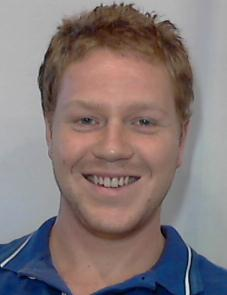
\includegraphics[height=6cm]{francois}
	\end{figure}
\end{center}

\section*
{
	\Huge{Francois Oberholzer}
}
\vspace{0.5cm}

\section*{Contact}
	\begin{description}
		\item[E-Mail:] u12039803@tuks.co.za
		\item[Cell:] (+27) 79 525 6883
	\end{description}

\section*{Skills}

	\subsection*{Programming}
		\begin{description}
			\item[c++:]Solid, 3 years practical experience
			\item[Java:]Solid, 2 years practical experience
			\item[Delphi]Moderate, 2 years practical experience
            \item[Php:]Limited, less than 1 year practical experience
            \item[Assembly]Limited, less that 1 year practical experience
		\end{description}
	\subsection*{Databases}
		\begin{description}
			\item[SQL Server:]Moderate, 2 years practical experience
		\end{description}
	\subsection*{Web}
		\begin{description}
			\item[HTML,CSS,JavaScript:]Solid, 3 years practical experience
			\item[jQuery]Limited, less than 1 year practical experience
			\item[JEE]Limited, less than 1 year practical experience
		\end{description}
	\subsection*{Other}
		\begin{description}
			\item[Joomla!]Moderate, created site at http://crossovertransformation.co.za/
            \item[Unity Game Engine]Limited, I have been playing with it for a year now
		\end{description}

\section*{Experience}

	\subsection*{2012}
		In my first year after finishing matric with 8 distinctions I got accepted to study BSc Computer Science at the University of Pretoria. 
	\subsection*{2013}
		During my second year of study, I was elected to the Residence Management Committee at TuksVillage Residence and served on this committee for one year. I completed the JCP Community Module as part of my course, creating a series of YouTube videos titled "The Ginger Chef", for which my group and I got awarded the "Best New Project". I helped out an overworked friend who designs websites for companies by doing the above mentioned Joomla! site.
	\subsection*{2014 - present}
		I develop an interest in Philosophy, and change by degree to BSc Information and Knowledge systems, so that I can double mayor in both Computer Science and Philosophy without being set back a year or two academically. I also started a Philosophy blog at http://sentivita.blogspot.com/. I am very thankful for the opportunities I have had to get to where I am.

\section*{Other Information}

	\subsection*{My Career Plan}

	 I have a very large interest in Artificial Intelligence, Human Consciousness and the link between them. I would like to continue my studies in both Computer Science and Philosophy, doing research and lecturing at a University. I aim to find what it is that makes Human Consciousness different from animal or other Consciousness, and bridge this gap, if possible, with Artificial Consciousness. I would also like to be an author and indie game designer in my spare time.

	\subsection*{Interests}

	I am fascinated by the human ability to think with intuition. I love AI, Philosophy and Psychology. I am also a lover of literature and music, playing piano and the tin whistle and writing a novel in my free time. I love language, and intend to learn many, but it is a slow process. I like games, and wish to have the time and resources to develop some of the ideas I have. Education also concerns me, and I wish to one day see the education system reformed to produce better results. This includes a reform of the current school curriculum as well as access to free, good quality education for all citizens. I hope to one day do something remarkable in each of these very different fields, and live a life that at least made a dent in the huge history of mankind.
\end{document}